%%%% ijcai11.tex

\typeout{IJCAI-13 Instructions for Authors}

% These are the instructions for authors for IJCAI-13.
% They are the same as the ones for IJCAI-11 with superficical wording
%   changes only.

\documentclass{article}
% The file ijcai13.sty is the style file for IJCAI-13 (same as ijcai07.sty).
\usepackage{ijcai13}

% Use the postscript times font!
\usepackage{times}

% the following package is optional:
%\usepackage{latexsym} 

\usepackage{amsthm}
\usepackage{amsmath}
\usepackage{amsfonts}
\usepackage{algpseudocode}
\usepackage{algorithm}
\usepackage{graphicx}

\newtheorem{theorem}{Theorem}
\newtheorem{definition}{Definition}
\newtheorem{corollary}{Corollary}
\newtheorem{lemma}{Lemma}
\newtheorem{proposition}{Proposition}

% Following comment is from ijcai97-submit.tex:
% The preparation of these files was supported by Schlumberger Palo Alto
% Research, AT\&T Bell Laboratories, and Morgan Kaufmann Publishers.
% Shirley Jowell, of Morgan Kaufmann Publishers, and Peter F.
% Patel-Schneider, of AT\&T Bell Laboratories collaborated on their
% preparation.

% These instructions can be modified and used in other conferences as long
% as credit to the authors and supporting agencies is retained, this notice
% is not changed, and further modification or reuse is not restricted.
% Neither Shirley Jowell nor Peter F. Patel-Schneider can be listed as
% contacts for providing assistance without their prior permission.

% To use for other conferences, change references to files and the
% conference appropriate and use other authors, contacts, publishers, and
% organizations.
% Also change the deadline and address for returning papers and the length and
% page charge instructions.
% Put where the files are available in the appropriate places.

\title{Game-Theoretic Question Selection for Tests}
%\author{Francesca Rossi \\
%University of Padova\\
%Italy \\
%pcchair13@ijcai.org}

\begin{document}

\maketitle

\begin{abstract}
Conventionally, the questions on a test are assumed to be kept secret
from test takers until the test.  However, for tests that are taken on
a large scale, particularly asynchronously, this is very hard to
achieve.  For example, example TOEFL iBT and driver's license test
questions are easily found online.  This also appears likely to become
an issue for Massive Open Online Courses (MOOCs).

In this paper, we take the loss of confidentiality as a fact.  Even
so, not all hope is lost as the test taker can memorize only a limited
set of questions, and the tester can randomize which questions appear on
the test.  We model this as a Stackelberg game, where the tester
commits to a mixed strategy and the follower responds.  We provide an
exponential-size linear program formulation, prove several NP-hardness
results, and give efficient algorithms for special cases.
\end{abstract}

\section{Introduction}

\section{Definitions and Notation}

%vc: change \mathbb B to \Theta 

A \emph{test game} $G = (Q, \Theta, p, t, u_1, u_2)$ is a 2-player
Bayesian game
between the tester (player 1) and the test taker (player 2). 
The tester has a set of potential test
questions $Q = \{q_1, q_2, \ldots, q_n\}$.\footnote{In common parlance,
  ``problem'' may be a better word, but this runs the risk of confusion
  with the computational problems studied in the paper.}
  The test taker has a type
$\theta \in \Theta$ ($|\Theta| = L$) that characterizes which questions
are hard for the test taker
 (i.e., which questions he would
not be able to answer without memorizing them), and how many questions the test
taker can memorize.  That is, $\theta = (H_\theta, m_\theta)$, where
$H_\theta \subseteq Q$ is the set of questions that are hard for $\theta$,
and $m_\theta \in \mathbb N$ is the number of questions for which $\theta$
would be able to memorize the answer, so that a test taker of type $\theta$
has $|H_\theta| \choose m_\theta$ pure courses of action.
(W.l.o.g., $m_\theta \leq |H_\theta|$.)
%and the test taker has an
%uncertain type (thus Bayes) characterized by $\mathbb B = \{B_1, B_2, \ldots,
%B_L\}$. Set $B_l \subseteq A$ is the unsolvable problem set of the $l$-th type
%test taker.  
$p: \Theta \rightarrow [0,1]$ is the
probability distribution over types.
% The memorize capacity
%function $m: \mathbb B \rightarrow \mathbb N$ denotes how many problems a
%particular test taker can memorize and the value function $v: \mathbb B
%\rightarrow \mathbb R^+$ denotes how much utility the tester gets if that test
%taker failed the test (recall that the tester can only fail test takers who
%cannot solve all problems and he want to fail as many of them as
%possible). 
%For
%simplicity, we write $p(B_l), m(B_l), v(B_l)$ as $p_l, m_l, v_l$ when the
%context is clear.  
The tester can put $t$ questions on the test, and thus has $n \choose t$
pure strategies.  We use $T$ to denote such a pure strategy, and $M_\theta$
to denote the subset of questions that $\theta$ memorizes.  $u_1(\theta, T,
M_\theta)$ denotes the tester's utility for type $\theta$, and $u_2(\theta,
T, M_\theta)$ denotes the utility of a test taker of type $\theta$.

In general, the utility functions could be very rich, depending in a
complicated way on the true type and the number (or even precise set) of
questions answered correctly.  To avoid getting too deeply into the
modeling aspects of this, we study only a special case that should be a
special case of most reasonable models.  This strengthens the hardness
results that we obtain later in the paper (since these hardness results
automatically also apply to the richer models of which our model is a
special case), though it weakens our positive results.  Specifically, we
assume that the only two outcomes of the test are to pass or fail the test
taker.  Moreover, we assume that the tester does not want to pass any test
taker that cannot answer all the questions (without memorizing any).  Thus,
the tester will pass exactly the agents that answer all the questions on
the test correctly.  Agents that can answer all the questions without
memorizing any have no strategic decisions to make and will always pass;
therefore, we do not model them explicitly as a type in the game.  (They
can be thought of as adding a constant to the tester's utility function
that is sufficiently large that the tester indeed wants to pass agents that
answer all questions correctly.)  

Thus, for the explicitly modeled types
$\theta$ (which the tester wants to fail), we assume that $u_1(\theta, T,
M_\theta) = 0$ if $T \cap (H_\theta \setminus M_\theta) \neq \emptyset$
(i.e., a question is tested that the agent cannot answer, so the 
the agent fails) and $u_1(\theta, T, M_\theta) = -v_\theta$ otherwise
(the cost of passing an agent of type $\theta$).  For the test takers,
$u_2(\theta, T,
M_\theta) = 0$ if $T \cap (H_\theta \setminus M_\theta) \neq \emptyset$,
and $u_2(\theta, T, M_\theta) = \omega_\theta$ otherwise.  Naturally, we require
$v_\theta >0$ and $\omega_\theta>0$.

%During the test, $t$ out of $n$ problems will be tested and
%a particular test taker will pass the test if all tested problems are either
%not in the unsolvable problem set or memorized.  

%The game only has two outcomes, pass or fail. The tester gets $0$ utility if a
%test taker passes and he gets $v_l$ utility if a type-$l$ test taker fails. On
%the type-$l$ test taker's side, he gets $0$ utility if he passes and $-v_l$ if
%he fails. From the test taker's perspective, any utility function that has a
%higher pass utility than fail utility will give him the same incentive to pass
%the test at his best. We define them as $0, -v_l$ specifically for the zero-sum
%property of the game.

%Our goal is to find the optimal strategy for the tester to maximize his utility
%under Stackelberg settings. 


We believe that a Stackelberg model is most natural for our setting, where
the tester first commits to a mixed strategy, and the test takers observe
this mixed strategy and best-respond.  This is because the test takers can
observe and learn the tester's strategy over time.  Arguably, however, if
the test takers are not able to do such learning, a Nash equilibrium model
(i.e., no Stackelberg leadership) also makes sense.  In the next section,
we show that in fact, both of these models are equivalent to the same
zero-sum game.



%That is, the tester firstly reveals his strategy
%about how $t$ problems are picked to test, then the test taker chooses the best
%memorizing strategy. This corresponds to our confidential-free assumption where
%test takers know what problems might be tested, their answers, and how likely
%they are tested. The only constraint for test takers is that they cannot
%memorize too many (greater than $m_l$) problem answers. 


\section{Equivalence to a Zero-Sum Game}

For any test game $G$ as defined above, we can modify it into a zero-sum
game $G'$ by substituting the following utility function for the test
taker: $u_2'(\theta, T, M_\theta) = 0$ if $T \cap (H_\theta \setminus
M_\theta) \neq \emptyset$, and $u_2'(\theta, T, M_\theta) = v_\theta$
otherwise.

\begin{proposition}
  The set of Stackelberg mixed strategies for the tester in $G$ is equal to
  the set of maximin strategies for the tester in $G'$.  These sets are
  also equal to the set of Nash equilibrium strategies for the tester in
  $G$.
\label{prop:equivalence}
\end{proposition}
\begin{proof}
First, we argue that the sets of Stackelberg mixed strategies for the
tester in $G$ and $G'$ are the same.  This follows from the fact that every
test taker type simply acts to maximize his probability of passing, whether
the utility function is $u_2$ or $u_2'$.  Second, it is well known that in
a 2-player zero-sum game, the set of Stackelberg mixed strategies is equal
to the set of maximin strategies for the leader.

Similarly, the sets of Nash equilibrium strategies for the
tester in $G$ and $G'$ are the same.  This again follows from the fact that every
test taker type simply acts to maximize his probability of passing, whether
the utility function is $u_2$ or $u_2'$.  Finally, it is well known that in
a 2-player zero-sum game, the set of Nash equilibrium strategies is equal
to the set of maximin strategies for the leader (by the minimax theorem~\cite{Neumann28:Zur}).
\end{proof}

We note that the equivalence to this zero-sum game is not complete, in the
sense that it would {\em not} hold if the {\em test taker} is a Stackelberg
leader who can commit to a strategy (before learning his type).  An example
is provided in Appendix~\ref{se:counterexample}.  However, since this
reversed Stackelberg model is not of primary interest to
us, we proceed with the zero-sum formulation from here on, focusing on $G'$
knowing that its solution will give us a solution to our original problem.


\section{General Linear Program (LP) Formulation}

Computing an optimal Stackelberg mixed strategy in a general 2-player
Bayesian game is NP-hard~\cite{Conitzer06:Computing} (in fact,
inapproximable~\cite{Letchford09:Learning}); a general mixed-integer linear
program formulation has previously been
proposed~\cite{Paruchuri08:Playing}.
%in terms of game matrix
%size so previous work used mixed integer LP (e.g. DOBSS [cite]) to solve them.
However, thanks to Proposition~\ref{prop:equivalence}, we only need to
solve for a maximin strategy of a zero-sum game.  The following linear
programming approach is standard:
%We model test games as zero-sum so we can bypass the NP-hardness and use the
%following maximin LP to solve our 2-player zero-sum Bayes Stackelberg games in
%polynomial time with respect to the game matrix size:

\begin{align}\label{eqn:maximin}
	\max~ &\sum_l p(\theta) V_\theta \\
	s.t. \ &(\forall \theta, \forall M_\theta \subseteq H_\theta
        : |M_\theta| = m_\theta)\nonumber\\
	&~~ \sum_{T \subseteq Q: |T| = t} \text  u_1(\theta, T, M_\theta) x_T \geq V_\theta;\nonumber\\
	&\sum_{T \subseteq Q: |T| = t} x_T = 1;\nonumber\\
	&(\forall T \subseteq Q: |T| = t) \  x_T \geq 0;\nonumber
\end{align}

Here, $V_\theta$ is the utility that the tester receives from type
$\theta$, and $x_T$ is the probability of testing exactly the questions in
$T$.
 %
%\begin{itemize}
%
% \item $V_l$: utility that the test taker can get from type $l$ test takers
%
% \item $C_l$: action space of type $l$ test takers, i.e. all combinations of
% problems that they can memorize.
%
% \item $R$: action space of the tester, i.e. all combinations of problems that
% he can test.
% 
% \item $x_r$: probability to test problem set $r$
%\end{itemize}

The dual of the above LP is:

\begin{align}\label{eqn:dual-original}
  \min~&U\\
  s.t. \ &(\forall T \subseteq Q: |T| = t)\nonumber\\
	&~~  U \geq \sum_{\theta, M_\theta
    \subseteq H_\theta : |M_\theta| = m_\theta} u_1(\theta, T, M_\theta) y_{\theta, M_\theta};\nonumber\\
  &(\forall \theta) \sum_{M_\theta \subseteq H_\theta : |M_\theta| =
    m_\theta} y_{\theta, M_\theta} = p(\theta);\nonumber\\
  &(\forall \theta, M_\theta \subseteq H_\theta : |M_\theta| = m_\theta) y_{\theta, M_\theta} \geq 0; \nonumber
\end{align}

%which is equivalent to 
%\begin{align}\label{eqn:minimax}
%  \min~&\max_r(U_r)\\
%  s.t. &(\forall r) U_r = \sum_{l, c_l} u^l(r, c_l) y_{l, c_l}\nonumber\\
%  &(\forall l) \sum_{c_l} y_{l, c_l} = p_l\nonumber\\
%  &(\forall l, c_l) y_{l, c_l} \geq 0\nonumber
%\end{align}

The variables of the dual LP $y_{\theta, M_\theta}$ give a strategy
for the test taker that maps types to probabilities of memorizing subsets
of questions: the probability of memorizing $M_\theta$ conditional on
having type $\theta$ is $y_{\theta, M_\theta} / p(\theta)$. 
$U = \max_{T \subseteq Q: |T| = t} U_T$  is the best-response utility for
the tester, 
 where $U_T = \sum_{\theta, M_\theta
    \subseteq H_\theta : |M_\theta| = m_\theta} u_1(\theta, T, M_\theta)
  y_{\theta, M_\theta}$ is the utility of testing $T$.  By linear
  programming duality, the two LPs have the same optimal
  solution value (corresponding to the minimax theorem); 
strategies corresponding to optimal solutions of these LPs
constitute an equilibrium of the game.

%The dual LP is as if that all types of test takers share the same goal to lower
%the tester's best testing utility ($\max_r (U_r)$ where $U_r$ is the utility of
%testing $r$) as much as possible by memorizing problems and revealling their
%memorizing strategies $y_{l, c_l}$ to the tester. This also shows that a
%Stackelberg strategy is also a Nash equilibrium if test takers play the dual
%minimax strategy.

Linear programs can be solved in time polynomial in their
size~\cite{Khachiyan79}.
However, while the size of the LPs above is polynomial in the size of the
game matrix, it is nevertheless exponential in the size of the natural
representation of our test games.
% the input of our test
%games: the tester's 
The tester's pure strategy space is exponential in $t$ (the number of
questions to test) and space of pure courses of action for a test taker of
type $\theta$ is exponential in $m_\theta$ (the number of questions whose
answers he can memorize).  When $t$ and $\max_\theta m_\theta$ are constant, the LPs indeed
give us a polynomial-time algorithm.
%So those LPs only give us polynomial
%algorithms when $m_l, t$ are constant. 
But, can the test game be solved in polynomial time when either the number
of questions to test, the number of answers to memorize, or both are not
constant?

\section{Constant Memory Size}

In this section, we study the case where memory size ($\max_\theta
m_\theta$) is constant, but test size $t$ is not.
%In order to formally characterize \emph{test game}'s hardness, define
We first define a decision variant of our problem:

\begin{definition}[The \textsc{Optimal Test Strategy} problem]
Given a test game $G$ and a value $u$, the \textsc{Optimal Test Strategy}
problem is to decide whether the tester has a strategy that gives her
a utility of at least $u$ (when the test taker best-responds).
\end{definition}

\begin{proposition}
  When memory size ($\max_\theta m_\theta$) is constant, \textsc{Optimal
    Test Strategy} is in NP.
\label{prop:inNP}
\end{proposition}
\begin{proof}
  When $\max_\theta m_\theta$ is constant, the number of constraints (not
  counting the nonnegativity constraints on the variables) in
  LP~(\ref{eqn:maximin}) is polynomial.  Any LP has an optimal solution
  with a number of nonzero variables that is at most the number of
  constraints (not counting the nonnegativity constraints)---this follows,
  for example, from the simplex algorithm.  Hence, a subset of the
  variables of this LP of this size can serve as a certificate: we can
  solve the LP restricted to these variables in polynomial time, and check
  whether the optimal solution is at least $u$.
\end{proof}

We now prove that the problem is in fact NP-hard, even when the test taker
cannot memorize any problems!

\begin{theorem}\label{thm:test-hardness}
Even if the test taker cannot memorize any problems ($m_\theta = 0$) and $|H_\theta| = 2$ for all
$\theta \in \Theta$,
\textsc{Optimal
Test Strategy} is NP-hard.% when test size $t$ is non-constant.
\end{theorem}
\begin{proof}
We reduce from the 
\textsc{Vertex Cover} problem, in which we are given a graph $(V,E)$ and a
number $k$, and are asked whether there exists a subset of $k$ vertices such
that every edge is incident on at least one of these vertices.
For any instance of this problem, we construct an \textsc{Optimal Test
	Strategy} instance as follows.
% Given a graph $G = (V, E)$, construct a
%	test game $G'$ with problem set $A = V$.  
      Let $Q=V$.  For each edge $e = \{i, j\} \in E$, add one type of test
      taker $\theta_e$ whose hard question set $H_{\theta_e} = e$.  Let
      $p(\theta_e) = 1/|E|, v_{\theta_e} = 1$ and $m_{\theta_e} = 0$ for
      all $e \in E$.  Finally, let $t=k$ and $u = 0$.

If there exists a vertex cover, consider the tester strategy of testing
exactly these questions.  Then, every type will fail at least one question
and hence the test, resulting
in a utility of $0$ for the tester.

Conversely, if there exists a tester strategy that gives the tester a
utility of $0$, then every type passes the test with probability $0$ under
this tester strategy.  Thus, consider any $T \subseteq Q$ with $|T| = k$ that
gets positive probability; every type must fail this test.  This means that
$T$ includes at least one endpoint of every edge, i.e., it is a vertex cover.
%Graph $G$ has a vertex cover of size $k$ if and only if the
%	tester has a strategy to test $t = k$ problems and gets $u=1$ utility
%	(i.e. all test takers will fail for sure) in test game $G'$.
\end{proof}

\section{Constant Test Size}

In this section, we study the case where test size is constant, but memory
size is not.


\begin{proposition}
  When the test size ($t$) is constant, \textsc{Optimal
    Test Strategy} is in coNP.
\end{proposition}
\begin{proof}
  When $t$ is constant, the number of constraints (not counting the
  nonnegativity constraints on the variables) in
  LP~(\ref{eqn:dual-original}) is polynomial.  As in the proof of
  Proposition~\ref{prop:inNP}, this implies that a subset of the variables
  of this LP of the requisite size can serve as a certificate that $u$
  cannot be achieved:  we can
  solve the LP restricted to these variables in polynomial time, and check
  whether the optimal solution is strictly less than $u$.  If so, then by
  weak duality, it is impossible for the tester to obtain $u$ or more (and
  moreover, by strong duality, if it is not possible for the tester to
  obtain $u$ or more, such a certificate must exist).
%Any LP has an optimal solution
%  with a number of nonzero variables that is at most the number of
%  constraints (not counting the nonnegativity constraints)---this follows,
%  for example, from the simplex algorithm.  Hence, a subset of the
%  variables of this LP of this size can serve as a certificate: we can
%  solve the LP restricted to these variables in polynomial time, and check
%  whether the optimal solution is at least $u$.
\end{proof}


\begin{theorem}\label{thm:memorize-hardness}
Even if the test size $t$ is $2$ and there are only two types that can
memorize any answers, \textsc{Optimal Test Strategy} is
coNP-hard.
% when memorize capacity is non-constant.
\end{theorem}

\begin{proof}
  We reduce from the \textsc{Independent Set} problem, in which we are
  given a graph $(V,E)$ and a number $k$, and are asked whether there
  exists a subset of $k$ vertices such that no two of these vertices have
  an edge between them.  For any instance of this problem, we construct an 
\textsc{Optimal Test Strategy} instance that has a ``no'' answer if and
only if the \textsc{Independent Set} instance has a ``yes'' answer,
as follows.  
%instances to test games with test size $t=2$
%and ask the complementary question: is $u$ the highest utility that the tester
%can get. That question has a yes answer if and only if the dual minimax LP
%[reference] has a feasible solution with objective at most $u$. 
Let $Q=V$.
Construct $|E|+|V|+2$ test taker types, as follows:
\begin{itemize}
\item For each edge $e = (i, j) \in E$, add one test taker type $\theta_e$ with
$v_{\theta_e} = |\Theta|$, $H_{\theta_e} = \{i, j\}$, and $m_{\theta_e} = 0$.

\item For each vertex $i$, add one test taker type  $\theta_i$ with $v_{\theta_i} =
|\Theta| (d_{\text{max}}-d(i)), H_{\theta_i} = \{i\}$, and $m_{\theta_i} = 0$. Here
$d(i)$ is the degree of vertex $i$ and $d_{\text{max}} = 1 + \max_i d(i)$.

\item Add a single test taker type 
$\theta^*$ with $v_{\theta^*} =
|\Theta| \alpha \varepsilon, m_{\theta^*} = 2$ and $H_{\theta^*} = V$, where $\alpha =
\binom{|V|}{2} - |E|-\binom{k}{2}$ and $\varepsilon < 1$.
%(specifically,  $\varepsilon =$?????? is small enough).

\item Finally, add a single test taker type $\theta^{**}$ with $v_{\theta^{**}} =
|\Theta|  \varepsilon, H_{\theta^{**}} = V$, and $m_{\theta^{**}} = k$.
\end{itemize}
Let the test taker types occur with uniform probability $p=1/|\Theta|$, let
$t=2$, and
let 
$$u= (2-|V|)d_{\text{max}} + |E| - \frac{{V  \choose 2}-|E|-1}{{V \choose 2}-|E|}\varepsilon$$

%$$u =  \frac{2 d_{\text{max}} +\alpha \varepsilon +\varepsilon -\frac{{V  \choose 2}-|E|-1}{{V \choose 2}-|E|}\varepsilon}{|\Theta|}$$


%Then we
%show that deciding whether $u = (2 d_G + a\cdot \varepsilon)/L$ is an
%upper-bound 
%for the tester's utility, or equivalently whether we can find a
%dual solution with objective as low as $u = (2 d_G + a\cdot \varepsilon)/L$ in
%our dual minimax LP, is equivalent to finding a size-$k$ independent set in
%$G$. 


First, suppose there exists an independent set of size $k$.  We will
construct a strategy for the test taker, that is, a feasible solution to
LP~\ref{eqn:dual-original}, that results in a utility of at most 
$(2-|V|)d_{\text{max}} + |E| - \varepsilon < u$
%$\frac{2  d_{\text{max}} +\alpha \varepsilon}{|\Theta|} < u$
for the tester.  Let type $\theta^{**}$ choose (memorize the answers to)
the questions in the independent set (with probability $1$).  Let type
$\theta^*$ choose a pair of questions that do not have an edge between
them, and of which at least one is outside the independent set (and choose
such a pair uniformly at random).  The other types have memory size $0$.

If, in response to this strategy, the tester chooses a pair of questions
with an edge between them ($(i,j) \in E)$), then the types that fail are
$\theta_i, \theta_j, \theta^*, \theta^{**}$, and all the $\theta_e$ where
$e \in E, e \cap \{i,j\} \neq \emptyset$.  This results in a savings of
$2d_{\text{max}} - d(i) - d(j) + \alpha \varepsilon + \varepsilon + d(i) +
d(j) - 1 = 2d_{\text{max}} + (\alpha+1) \varepsilon - 1$ relative to
passing everyone.  If the tester chooses $i$ and $j$ with $(i,j) \notin E$
and at least one of $i$ and $j$ outside the independent set, then the types
that fail with probability $1$ are $\theta_i, \theta_j, \theta^{**}$, and
all the $\theta_e$ where $e \in E, e \cap \{i,j\} \neq \emptyset$; type
$\theta^*$ fails with probability $\frac{\alpha-1}{\alpha}$.  This results
in a savings of $2d_{\text{max}} - d(i) - d(j) + \varepsilon + d(i)+d(j) +
\frac{\alpha-1}{\alpha} \alpha \varepsilon = 2d_{\text{max}} + \alpha
\varepsilon$ (which is greater than the previous case).  Finally, if the
tester chooses $i$ and $j$ that are both in the independent set, then the
types that fail are $\theta_i, \theta_j, \theta^*$, and all the $\theta_e$
where $e \in E, e \cap \{i,j\} \neq \emptyset$.  This results in a savings
of $2d_{\text{max}} - d(i) - d(j) + \alpha \varepsilon + d(i) + d(j) =
2d_{\text{max}} + \alpha \varepsilon$ (which is the same as the previous
case).  Because the utility to the tester of passing everyone is $-|E| -
|V|d_{\text{max}} + 2|E| - \alpha \varepsilon - \varepsilon$, a savings of
$2d_{\text{max}} + \alpha \varepsilon$ results in a utility of
$(2-|V|)d_{\text{max}} + |E| - \varepsilon < u$ for the tester.  So the
answer to the \textsc{Optimal Test Strategy} instance is ``no.''


Conversely, suppose that no independent set of size $k$ exists.  Consider
the tester mixed strategy that chooses a pair of questions $i,j$ with
$(i,j) \notin E$ uniformly at random (there are ${|V| \choose 2} - |E|$
such pairs).  We will show that this strategy guarantees the tester an
expected utility of at least $u$.  Again, we will reason in terms of the
savings to the tester relative to passing everyone.  We first consider the
savings from types $\theta_e$ with $e \in E$ and $\theta_i$ with $i \in V$.
For these types (which do not have a choice to make), it is easier to
reason about the savings resulting from testing a specific pair of
questions $i,j$ with $(i,j) \notin E$ with probability $\frac{1}{{|V|
    \choose 2} - |E|}$.  This savings is $\frac{d(i)+d(j)+2d_{\text{max}} -
  d(i) - d(j)}{{|V| \choose 2} - |E|} = \frac{2d_{\text{max}}}{{|V| \choose
    2} - |E|}$.  Because there are ${|V| \choose 2} - |E|$
such pairs, we have a total savings of $2d_{\text{max}}$.
%The probability that a
%type $\theta_e$ with $e = (i,j) \in E$ fails is $\frac{2n-2-d(i)-d(j)}{{|V|
%    \choose 2} - |E|}$, so the total savings corresponding to these types
%is $\sum_{(i,j) \in E} \frac{2n-2-d(i)-d(j)}{{|V| \choose 2} - |E|} = \frac
%{(2n-2)|E| - \sum_i d(i)^2}{{|V| \choose 2} - |E|}$.  The probability that
%a type $\theta_i$ with $i \in v$ fails is $\frac{n-1 - d(i)}{{|V| \choose
%    2} - |E|}$, so the total savings corresponding to these types
%is  $\sum_{i \in V} (d_{\text{max}}-d(i)) \frac{n-1 - d(i)}{{|V| \choose
%    2} - |E|}$. 
The best response for type $\theta^*$ is to memorize any pair $\{i,j\}$
where $(i,j) \notin E$, 
%vc: maybe say $\{i,j\} \notin E$.
resulting in a probability of $\frac{{|V| \choose 2} - |E| - 1}
{{|V| \choose 2} - |E|}$ that this type fails, so the total savings
corresponding to this type is $\alpha \varepsilon 
\frac{{|V| \choose 2} - |E| - 1}
{{|V| \choose 2} - |E|} = \alpha \varepsilon (1-\frac{1}{{|V| \choose 2} - |E|})$
%$(\binom{|V|}{2} - |E|-\binom{k}{2})
%$\varepsilon 
%\frac{{|V| \choose 2} - |E| - 1}
%{{|V| \choose 2} - |E|}$.
Finally, because by assumption, no independent set of size $k$ exists, no
matter which set of $k$ problems $\theta^{**}$ memorizes, the probability
that $\theta^{**}$ fails is at least $\frac{{|V| \choose 2} - |E| - {k
    \choose 2} +1}{{|V| \choose 2} - |E|} = \frac{\alpha+1}{{|V| \choose 2}
  - |E|}$, so the total savings corresponding to this type is at least
$\varepsilon \frac{\alpha+1}{{|V| \choose 2} - |E|}$.  Summing the savings
for $\theta^*$ and $\theta^{**}$, we get $\alpha \varepsilon +
\frac{\varepsilon}{{|V| \choose 2} - |E|}$.
Adding all these savings to the utility to the tester of passing everyone,
which is  $-|E| -
|V|d_{\text{max}} + 2|E| - \alpha \varepsilon - \varepsilon$, 
we get that the tester's utility is $(2-|V|)d_{\text{max}} + |E| 
+ \frac{\varepsilon}{{|V| \choose 2} - |E|} -\varepsilon =
(2-|V|)d_{\text{max}} + |E| - \frac{{V  \choose 2}-|E|-1}{{V \choose
    2}-|E|}\varepsilon
= u$.
 So the
answer to the \textsc{Optimal Test Strategy} instance is ``yes.''
%
%Recall that a dual solution is a strategy for test takers to memorize
%problems. If no one memorizes, the tester's utility $U_r$ to test a problem set
%$r$ is $U_r = (2d_G+a\cdot\varepsilon + \varepsilon) /L$ if $r \notin E$ and
%$U_r = (2d_G-1+a\cdot\varepsilon + \varepsilon)/L$ if $r \in E$. To lower the
%objective, test takers $l_\alpha, l_k$ should memorize problem sets that bring
%the maximum of $U_r$ down.  No matter what the strategy is (as long as they
%only memorize unsolvable problems), $\sum_r U_r$ is a constant. And because
%$U_r$ for $r \notin E$ is much larger than $U_r$ for $r \in E$ as $\varepsilon
%\ll 1$, it's better to only decrease $U_r$ for $r \notin E$. The only way to do
%that is to let $l_\alpha$ test takers only memorize pairs of problems that are
%not edges and let $l_k$ test takers only memorize size-$k$ indepedent sets of
%problems.  If there's a size-$k$ independent set, let $l_k$ test takers
%memorize one size-$k$ independent set all the time and let $l_\alpha$ test
%takers memorize all pairs of problems that are not covered by that independent
%set with uniform probability. That will make $U_r = (2d_G+a\cdot\varepsilon)/L$
%for $r \notin E$ and $U_r = (2d_G-1+a\cdot\varepsilon+\varepsilon)/L$ for $r
%\in E$.  This is the best they can achieve and this can only be achieved when a
%size-$k$ independent set exists in $G$.
%
\end{proof}


%\subsection{Summary on General Test Games}
%
%\begin{theorem}
%The \textsc{Optimal Test Strategy} for a \emph{test game} can be computed in
%polynomial time when test size and memorize capacity are constant. It's
%NP-complete when test size is non-constant and coNP-complete when memorize
%capacity is non-constant. Hence it's both NP-hard and coNP-hard when both test
%size and memorize capacity are non-constant.
%\end{theorem}

%\begin{proof}
%When test size and memorize capacity are both non-constant, \textsc{Optimal
%Test Strategy} is both NP-hard and coNP-hard by Theorem~\ref{thm:test-hardness}
%and \ref{thm:memorize-hardness}.  LP~(\ref{eqn:maximin}) shows that
%\textsc{Optimal Test Strategy} can be computed in polynomial time when test
%size and memorize capacity are constant.  When memorize capacity is constant or
%test size is constant, either the primal LP~(\ref{eqn:maximin}) or the dual
%LP~(\ref{eqn:dual-original}) has constant number of constraint. Such LP has a
%polynomial size optimal solution even if the number of variables is
%exponential. That optimal solution's feasibility and objective can be checked
%in polynomial time. Therefore \textsc{Optimal Test Strategy} is in NP when
%memorize capacity is constant and it is in coNP when test size is constant.
%Hence they are NP-complete and coNP-complete respectively by
%Theorem~\ref{thm:test-hardness} and \ref{thm:memorize-hardness}. 
%\end{proof}



%[COMPLEXITY TABLE AT END OF PAPER]

\section{Tests of Size One}

%We showed the hardness of test games when either one of test size or memorize
%capacity is non-constant. 
Theorem~\ref{thm:test-hardness} shows that when we do not bound the test
size, our problem is hard even if test takers cannot memorize anything.
%the test size is non-constant, there is little
%we can improve because it is NP-hard even if the memorize capacity is zero.
But, if we do not bound the memory size,
Theorem~\ref{thm:memorize-hardness} only shows that our problem is hard if
the tester can test two questions simultaneously.  
%When the memorize capacity is non-constant, our proof for
%Theorem~\ref{thm:memorize-hardness} only showed that NP-hardness for testing 2
%problems. 
This still leaves open whether an efficient algorithm exists when the test
size is restricted to $1$.  In this section, we show that this is in fact
the case.  Our interest in this special case derives not only from it being
left open by our hardness results, but also from potentially important
applications.  For one, an interviewer often only has time to ask an
applicant a single question.  Moving away from interpreting questions
literally, a (for example) nuclear inspections team may be able only to
inspect a single site (within a particular time frame).

In this special case, LP~(\ref{eqn:maximin}) has polynomially many
variables, but an exponential number of constraints.  A quick proof of the
polynomial-time solvability of this case is given by establishing that
there is a polynomial-time separation oracle for finding a violated constraint.
This separation oracle is straightforward: simply select, for every type
$\theta$, the $m_\theta$ problems in $H_\theta$ that get the highest
probability $x_q$ in the current solution (breaking ties arbitrarily), and
see whether the corresponding constraint is violated.  However, in this
section, we develop more direct approaches that do not require generating
violated constraints and that give more insight into the structure of the solution.
%A quick evidence for the existence of such polynomial algorithm is
%constraint generation. Though there are exponential many constraints, we can
%find the most violated constraint in polynomial time by: enumerate over all
%types of test takers; for type-$l$ test takers  select top $m_l$ problems $M_l$
%according to $x_a$ that maximize $\sum_{a \in M_l} x_a$; finally see whether
%$V_l - \sum_{a \in B_l \backslash M_l} x_a$ updates the most violated
%constraint.

%We also investigated such tests by conducting experiments using
%LP~(\ref{eqn:maximin}). Surprisingly, no matter how input varies, the strategy
%we get always has the following format: among a subset $T$ of problems $A$,
%test any one of them with uniform probability. That is counter-intuitive as
%some problems in $T$ seem to be obviously more superior than others so
%intuitively they should be tested with more probability. For example, when $n$
%problems can be sorted by difficulty, a test taker who can solve a harder
%problem can always solve an easier problem. In that case, it seems that the
%hardest problem should be tested strictly more likely than the second hardest
%problem. But in most cases, the optimal strategy will test one of them with
%equal probability.

%[EXAMPLE TABLE]

%Inspired by that uniform test property, we present an algorithm to compute
%optimal strategies and use it to prove uniform test property
%consequently. 

\subsection{Linear Program}

We first present a  linear program that can be thought of as a
polynomial-size version of LP~\ref{eqn:dual-original}.  Instead of 
variables $y_{\theta,M_\theta}$, this linear program has a variable
$z_{\theta,q}$ for every individual $q \in H_\theta$.  These variables
correspond to the {\em marginal} probability that $\theta$ memorizes $q$
(in this case, conditional on $\theta$ being the type).
In the case where the tester tests one question, these marginal
probabilities are all that matter.  (This is not true when the tester tests
more than one question, because in that case, for example, if the tester
always tests two questions together, a test taker may be best off
memorizing the answers either to both questions or to neither question.)
 Let
$U^0_q$ be the utility that the tester obtains when she tests $q$ and nobody
memorizes $q$, i.e., $U^0_a =
\sum_{\theta: q \notin H_\theta} p(\theta)(-v_\theta)$. 
%The algorithm's first part is based on
%the following LP:
\begin{align}\label{eqn:one-problem}
	\min~ &U\\
	s.t.~ &(\forall q \in Q)~ U \geq U^0_q - \sum_{\theta : q \in
          H_\theta} p(\theta)v_\theta z_{\theta,q}\nonumber\\
	&(\forall \theta \in \Theta)~ \sum_{q \in H_\theta} z_{\theta,q} \leq m_\theta\nonumber\\
	&(\forall \theta \in \Theta, q \in H_\theta)~ 0 \leq z_{\theta, q} \leq 1\nonumber
\end{align}
%It modifies LP~(\ref{eqn:dual-original}) by:
%\begin{enumerate}
%	\item Change joint probability $y_{l, c_l}$ to marginal probability
%	$z_{l, a}$ of memorizing one problem $a$.  We did this modification
%	because marginal probability is more meaningful for one-problem test
%	and we can always restore a joint probability from a marginal
%	probability[reference].
%	\item Relax equality $\sum_{a \in B_l} z_{l, a} = m_l$ to inequality
%	$\sum_{a \in B_l} z_{l,a} \leq m_l$ (allow using less memorize
%	capacity).  We can do this because $v_l \geq 0$ (thus $u^l, V_l \geq
%	0$) and this modification is essentially adding $V_l \geq 0$ to the
%	primal LP~(\ref{eqn:maximin}). Intuitively, memorizing less problems
%	won't hurt tester's utility.
%\end{enumerate}

%(The second-to-last constraint can equivalently be replaced with $\sum_{q
%  \in H_\theta} z_{\theta,q} = m_\theta$, but the inequality form will help
%us later on.)

Solving LP~(\ref{eqn:one-problem}) 
%vc: add parentheses elsewhere too
gives us an equilibrium test taker strategy.\footnote{To be precise, we have to
find a test taker strategy that has these marginal probabilities.
This is quite straightforward in this context: for example, one can, for
each question in sequence, flip a coin with the appropriate probability to
determine whether to memorize it, and subsequently renormalize the remaining
questions' probabilities to ensure that the (expected) number of memorized
questions stays the same.  This strategy, however, has an
exponential-size support and so the support cannot be listed explicitly.
Alternatively, we can find the mixed strategy
explicitly using the Dulmage-Halperin
algorithm~\cite{Dulmage55:Frobenius,Chang01:Birkhoff} for finding the
Birkhoff-von Neumann decomposition~\cite{Birkhoff46:Tres}; similar
techniques are used in the context of security
games~\cite{Korzhyk10:Complexity}.}
An equilibrium tester strategy can be read off from the corresponding
solution to the dual of this linear program. ?????APPENDIX???????


\subsection{A Network Flow Approach}


Our algorithm is shown in Algorithim~\ref{alg:one-problem}.

\begin{algorithm}
\caption{Compute the optimal one-problem test strategy}\label{alg:one-problem}
\begin{algorithmic}[1]
\Function{OptimalOneProblemTest}{$A, \mathbb B, m, v, p$}
	\State Solve LP~(\ref{eqn:one-problem}) and let the solution be $U, z_{l,a}$
	\State $T \gets \{a ~|~ U^0_a \geq U\}$
	\State $Q \gets $ all $B_l$ such that $\sum_{a \in B_l \cap T} z_{l,a} < m_l$
	\ForAll {$B_l \in Q$} \Comment{Potential Memorizing Power}
		\State $G(B_l) \gets m_l-\sum_{a \in B_l \cap T} z_{l,a}$ \label{line:first-potential}
	\EndFor
	\While{$Q$ has an unmarked element}
		\State $B_l \gets $ get and mark an unmarked element from $Q$
		\ForAll{$a \in B_l \cap T$ and $z_{l,a} < 1$}
			\State $T \gets T \backslash \{a\}$\label{line:delete-a}
			\ForAll {$B_{l'} \ni a $ and $z_{l', a}>0$}
				\State $G(B_{l'}) \gets \min(z_{l',a}, \frac{G(B_l)}{|B_l|L})$\label{line:second-potential}
				\State Push $B_{l'}$ into $Q$\label{line:second-push}
			\EndFor
		\EndFor
	\EndWhile
	\State \Return{Strategy that test $T$ uniformly}
\EndFunction
\end{algorithmic}
\end{algorithm}

We prove the correctness of Algorithm~\ref{alg:one-problem} by firstly introducing the
following two lemmas.

\begin{lemma}\label{lemma:non-empty}
$T$ returned by Algorithm~\ref{alg:one-problem} is non-empty.
\end{lemma}
\begin{proof}
$T$ is non-empty before we delete problems from $T$ on line~\ref{line:delete-a}
of Algorithm~\ref{alg:one-problem}.  Denote that initial $T$ as $T_0$.  If all
problems in $T_0$ are deleted, then for every $a$ in $T_0$ there is a $B_l$
that is in $Q$ and $z_{l,a} < 1$.  Note that for every $B_l$ in $Q$, it has a
positive potential memorizing power $G(B_l)$ either because $\sum_{a \in B_l}
z_{l,a} < m_l$ (on line \ref{line:first-potential}) or because there is an
unnecessary memorizing $z_{l, a} > 0$ that can be freed (on line
\ref{line:second-potential}). This means that we can bring $U$ down by using
those potential memorizing powers to memorize every problem in $T_0$ more
(recall that $z_{l,a} < 1$), a contradiction to that $U$ is minimized.
\end{proof}

\begin{lemma}\label{lemma:best-response}
Let $z_{l,a}$ be the solution of LP~(\ref{eqn:one-problem}) and $T$ be the final
subset that Algorithm~\ref{alg:one-problem} returns. Then for each type of test
takers $B_l$, either $\sum_{a \in B_l \cap T} z_{l,a} = m_l$ (they memorize a
subset of $T$ that are unsolvable all the time) or $\forall a \in B_l \cap T,
z_{l, a} = 1$ (they memorize unsolvable problems in $T$ all the time so they
will pass the test for sure).
\end{lemma}
\begin{proof}
Let $T_0$ be the initial $T$ before any deletion on line~\ref{line:delete-a} of
Algorithm~\ref{alg:one-problem}.  Initially, for any $B_l$ such that $\sum_{a
\in B_l cap T_0} z_{l,a} < m_l$, we push it to $Q$. After that any $a \in B_l$
where $z_{l,a} < 1$ is deleted from $T$ on line~\ref{line:delete-a}. Therefore
$\forall a \in B_l \cap T, z_{l,a} = 1$ must hold for that $B_l$. Afterwards,
more $B_l$ may violate $\sum_{a \in B_l cap T} z_{l,a} < m_l$ because some $a$
are deleted from $T$.  But for those $B_l$, we must have pushed them into $Q$
on line~\ref{line:second-push}. So they will satisfy $\forall a \in B_l \cap T,
z_{l,a} = 1$ afterwards. In the end, every $B_l \in Q$ will satisfy $\forall a
\in B_l \cap T, z_{l,a} = 1$ and every other $B_l \notin Q$ will satisfy
$\sum_{a \in B_l \cap T} z_{l,a} = m_l$.
\end{proof}

Then we show our strategy is optimal by complementary slackness theorem, which
in our context is essentially: 1) the tester only tests problems (non-zero
primal variables) that gives him best utility (tight dual constraints); 2) the
test taker only memorizes problems (non-zero dual variables) that gives him
best utility (tight primal constraints).\footnote{This is essentially saying
that in a zero-sum game, a minimax, or maximin state is reached, if and only if
the Nash equilibrium is reached.} We will need two more lemmas as follows to
use the complementary slackness theorem.

\begin{theorem}
Uniformly testing $T$ returned by Algorithm~\ref{alg:one-problem} is optimal.
\end{theorem}
\begin{proof}
First of all, $T$ is non-empty by Lemma~\ref{lemma:non-empty} so we can test
$T$ uniformly. Then since memorizing strategy $z_{l,a}$ makes $U_a$ (the
utility to test a problem $a$) decrease to $U$ if $U^0_a > U$ and we only pick
$T$ from problems that $U^0_a > U$, every problem that we might test gives the
tester best utility. That is the first condition for the complementary
slackness theorem.  Finally, Lemma~\ref{lemma:best-response} shows that one
type of test takers either pass the test for sure or memorize a subset in $T$
all the time which is optimal for uniform test, the second condition of
complementary slackness theorem holds.
\end{proof}

Finally, instead of using general LP algorithm like simplex [cite] to solve
LP~(\ref{eqn:one-problem}), we can alternatively use binary search plus max
flow to solve it as shown in Algorithm~\ref{alg:max-flow}.  With a given $U$,
we use max flow to check its feasibility. Intuitively, a $U$ is feasible if and
only if there is a strategy $z_{l, a}$ such that for every $a$ where $U^0_a >
U$, that strategy decreases it down to $U$. This is achievable if and only if
the max flow can saturate all edges from $A$ to $t$. Given a max flow $f$, we
can restore the strategy by setting $z_{l, a} = f_{(B_l, a)}/c_{(B_l, a)}$
which is the flow of an edge divded by the capacity of an edge. If we use
Push-Relabel algorithm [cite] to solve the max flow in $O((n+L)^3)$ time, the
whole Algorithm~\ref{alg:one-problem} runs in $O((n+L)^3 + \sum_l |B_l|)$ time
as the remaining part can run in linear time with repsect to the input size
(assuming we only binary search for constant times to achieve a constant
accuracy).

\begin{algorithm}
\caption{Use binary search and max flow to solve LP~(\ref{eqn:one-problem})}
\label{alg:max-flow}
\begin{algorithmic}[1]
	\State $U_{lower} \gets 0, ~U_{upper} \gets \max_{a \in A} U^0_a$
	\While{$U_{upper}-U_{lower} > \epsilon$}\Comment{Binary search}
		\State $U \gets (U_{upper}+U_{lower})/2$ \Comment{Objective utility}
		\State $V \gets \{s\} \cup \mathbb B \cup A \cup \{t\}$ \Comment{Vertex set}
		\State $E \gets \emptyset$ \Comment{Initialize edge set}
		\ForAll{$a \in A$}
			\If{$U^0_a > U$}
				\State $E \gets E \cup \{(a, t)\}$
				\State $c_{(a, t)} \gets U^0_a-U$ \Comment{Edge capacity}
			\EndIf
		\EndFor
		\ForAll{$B_l \in \mathbb B$} 
			\State $E \gets E \cup \{B_l\} \times B_l$ %\Comment{Edges between $\mathbb B$ and $A$}
			\State $c_{\{B_l\} \times B_l} \gets p_l v_l$ 
			\State $E \gets E \cup \{(s, B_l)\}$ %\Comment{Edges between $\{s\}$ and $\mathbb B$}
			\State $c_{(s, B_l)} \gets p_l m_l v_l$
		\EndFor
		\State $f \gets \Call{MaxFlow}{G = (V, E), c}$
		\If{$f$ saturates all edges in $A \times \{t\}$}
			\State $U_{upper} \gets U$
		\Else
			\State $U_{lower} \gets U$
		\EndIf
	\EndWhile
	\State $(\forall l, a), z_{l,a} \gets f_{(B_l,a)} / c_{(B_l, a)}$
	\State \Return{$U, z_{l,a}$}
\end{algorithmic}
\end{algorithm}

\subsection{Experiments}

In this section, we conduct experiments to see how different approaches scale
on one-problem test games. The first approach is using CPLEX to solve our
general LP~(\ref{eqn:maximin}) which is exponential to the memorize capacity.
The second one is using CPLEX to directly solve the marginal version
LP~(\ref{eqn:one-problem}).  The third and fourth use
Algorithm~\ref{alg:max-flow} to solve LP~(\ref{eqn:one-problem}). They are
using Edmonds-Karp [cite] and Psh-Relabel\footnote{We modified its is\_flow
function for floating number issues.} [cite] max flow algorithm in C++ boost
library respectively.

%Therefore
%we focused on comparing different varieties of
%Algorithm~\ref{alg:one-problem}. In high level, there are two different
%ways to implement: one is solving LP~(\ref{eqn:one-problem}) using general LP
%algorithm and the other is solving it using max flow as shown in
%Algorithm~\ref{alg:max-flow}. In low level, we compared glpk and cplex for
%general LP solving methods and compared Edmonds-Karp [cite] and
%Push-Relabel\footnote{We modified its is\_flow function for floating number
%issues.} [cite] using C++ boost library [cite] for max flow methods.  In
%summary, we have four varieties in our comparisons.

For each test case, we specify four parameters $n, L, m_{max}, b_{max}$,
the number of problems, the number of test taker types, the maximum memorize
capacity and the maximum size of $B_l$. Given those parameters, a test game
instance is generated as follows: for each $1 \leq l \leq L$, generate $m_l$
uniformly from $1$ to $m_{max}$, generate $|B_l|$ uniformly from $m_l$ to
$b_{max}$, generate $B_l$ by selecting $|B_l|$ elements from $A$ uniformly and
generate $w_l = v_l p_l$ (weight of type-$l$) from $[0,1]$ uniformly. Here we
only generate $w_l$ because $v_l$ and $p_l$ always appear together as $v_l
p_l$. For each parameter setting, we generate $5$ test game instances and
compute the average running time for each algorithm. During each run, we set
timeout to 5 seconds. 

\begin{figure}
	\caption{Average running time (timeout after 5 seconds) for different
	one-problem test algorithms over the number of problems $n$. For each
	$n$, we set the other three parameters $L = n, m_{max} = \lfloor
	\sqrt{n} \rfloor$ and $b_{max} = 2m_{max}$ (see
	Table~\ref{tab:settings}).}
	\label{fig:benchmark}
	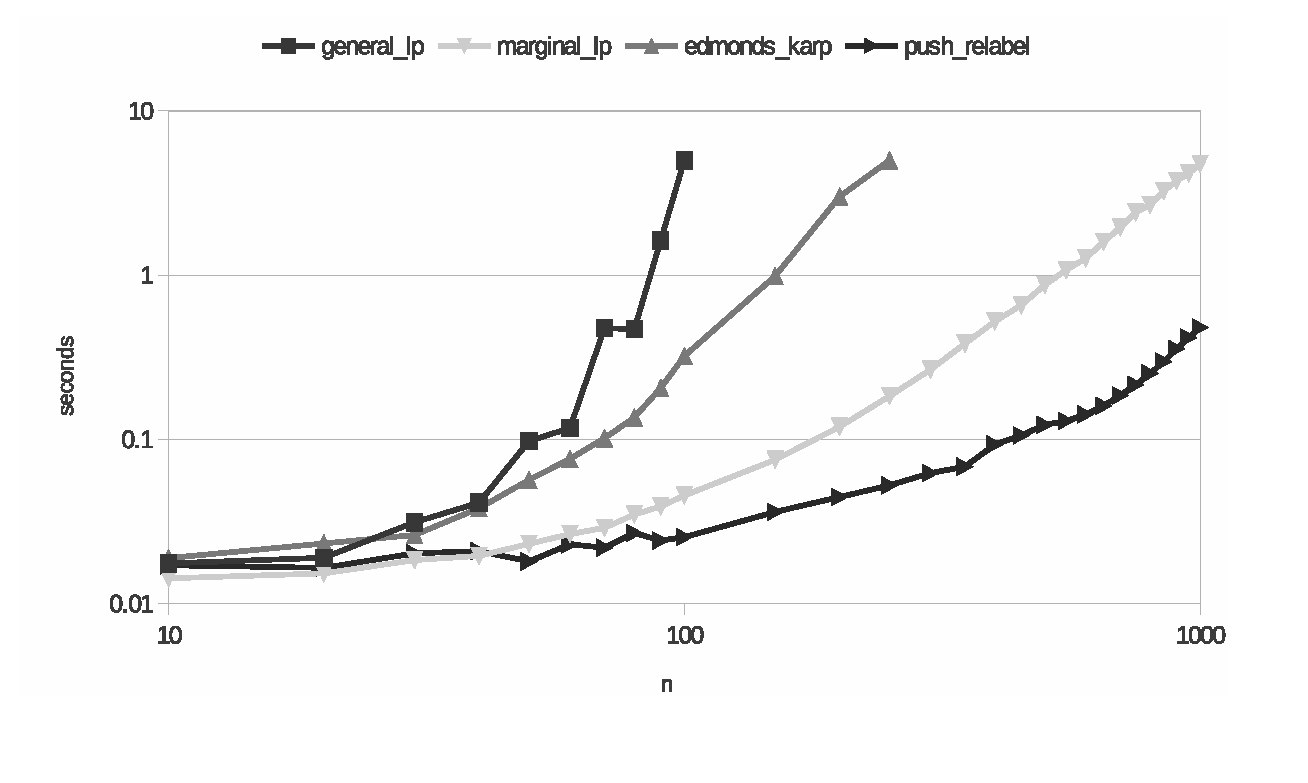
\includegraphics[trim=0 10mm 0 -5mm, clip, width=\linewidth]{benchmark_all}
\end{figure}

In our benchmark, we increase $n$ and set the remaining three parameters $L,
m_{max}, b_{max}$ as following: $L = n, m_{max} = \lfloor \sqrt{n} \rfloor$ and
$b_{max} = 2m_{max}$. Note that our $L, b_{max}$ are quite small (they can be
as large as $b_{max} = n/2, L = \binom{n}{b_{max}})$. That's becuase for large
$L, b_{max}$, our uniform random input will almost always make the trivial
strategy to uniformly test among all $n$ problems optimal. So we make them
small to avoid such trivial solutions. The realized parameter settings are
shown in Table~\ref{tab:settings}. The benchmark is shown in
Figure~\ref{fig:benchmark}.  As expected, the general LP is exponential so it
times out before $n$ reaches $100$.  Unexpectedly, using CPLEX to directly
solve LP~(\ref{eqn:one-problem}) is much faster than Edmonds-Karp
implementation. Finally, Push-Relabel version outperforms all others
significantly. It solves $n=1000$ case in about $0.5$ second while the second
best CPLEX version uses almost 5 seconds.

[Machine, GLPK and GPLEX spec]

\begin{table}
	\caption{Parameter settings for the benchmark}\label{tab:settings}
	\begin{center}
	\begin{tabular}{ r r r r }
		$n$&$L$&$m_{max}$&$b_{max}$\\
		\hline\\
		10&	10&	3&	6 \\ 
%		20&	20&	4&	8 \\
%		30&	30&	5&	10\\
%		40&	40&	6&	12\\
		50&	50&	7&	14\\
%		60&	60&	7&	14\\
%		70&	70&	8&	16\\
%		80&	80&	8&	16\\
%		90&	90&	9&	18\\
		100&100&10&20\\
%		150&150&12&24\\
%		200&200&14&28\\ 
%		250&250&15&30\\
		300&300&17&34\\
%		350&350&18&36\\
%		400&400&20&40\\
%		450&450&21&42\\
		500&500&22&44\\
%		550&550&23&46\\
%		600&600&24&48\\
%		650&650&25&50\\
		700&700&26&52\\
%		750&750&27&54\\
%		800&800&28&56\\
%		850&850&29&58\\
%		900&900&30&60\\
%		950&950&30&60\\
		1000&1000&31&62
	\end{tabular}
	\end{center}
\end{table}


\section{Conclusion}

%\section*{Acknowledgments}


\appendix

\section{Counterexample to Zero-Sum Equivalence When the Test Taker Is the
  Stackelberg Leader}
\label{se:counterexample}

Let $Q=\{q_1,q_2\}$, $\Theta=\{\theta_1,\theta_2\}$,
$H_{\theta_1}=H_{\theta_2}=Q$, $m_{\theta_1}=m_{\theta_2}=1$,
$p(\theta_1)=p(\theta_2)=1/2$, $t=1$, $v_{\theta_1} = 100$, $v_{\theta_2} =
1$, $\omega_{\theta_1} = 1$, and $\omega_{\theta_2} = 100$.  If the tester
is the leader, then it is optimal for her place probability $1/2$ on each
question (and so, by Proposition~\ref{prop:equivalence}, this is also
optimal in the zero-sum version of the game).  This results in an expected
utility of $0.5$ for a test taker of type $\theta_1$, and one of $50$ for a
test taker of type $\theta_2$---so an expected utility of $25.25$ for the
test taker {\em ex ante}.

However, if the test taker can commit to a strategy in the Bayesian game
{\em ex ante} (before learning his type), then he can commit to
memorize conditionally on the type as follows: $M_{\theta_1} =\{q_1\}$ and 
$M_{\theta_2} =\{q_2\}$.  Because the tester cares more about failing
$\theta_1$, she will test $q_2$.  This results in an {\em ex ante} expected
utility of $(1/2) \cdot 100 = 50$ for the test taker, which is more than
the $25.25$ from the strategy in the regular version.













\section{Dual of the linear program and interpretation}


%% The file named.bst is a bibliography style file for BibTeX 0.99c
\bibliographystyle{named}
\bibliography{/usr/project/conitzer/vccollab/references.bib}

\end{document}

